\documentclass[10pt,a4paper]{article}
\usepackage{esint} % also loads fontspec
%\usepackage{amsmath,amssymb}
\usepackage{nath}

\usepackage{amssymb}

%\delimgrowth=1
\usepackage{hyperref}
\hypersetup{
    colorlinks=false, %set true if you want colored links
    linktoc=all,     %set to all if you want both sections and subsections linked
    linkcolor=blue,  %choose some color if you want links to stand out
}

\usepackage[left=0.8in, top=0.5in, bottom=0.8in]{geometry}

%\usepackage{draftwatermark}
%\SetWatermarkText{Draft}
%\SetWatermarkScale{5}

%\usepackage{mathtools}
 
%\usepackage{amsmath}

%\addtolength{\oddsidemargin}{-.875in}
%\addtolength{\evensidemargin}{-.875in}
%\addtolength{\textwidth}{1.75in}

%\addtolength{\topmargin}{-1.1in}
%\addtolength{\textheight}{1.75in}

%\graphicspath{ {fig/} }
%\usepackage{graphicx}



\begin{document}
\section{Integrated Matching}

\begin{figure}[h!]
\centering
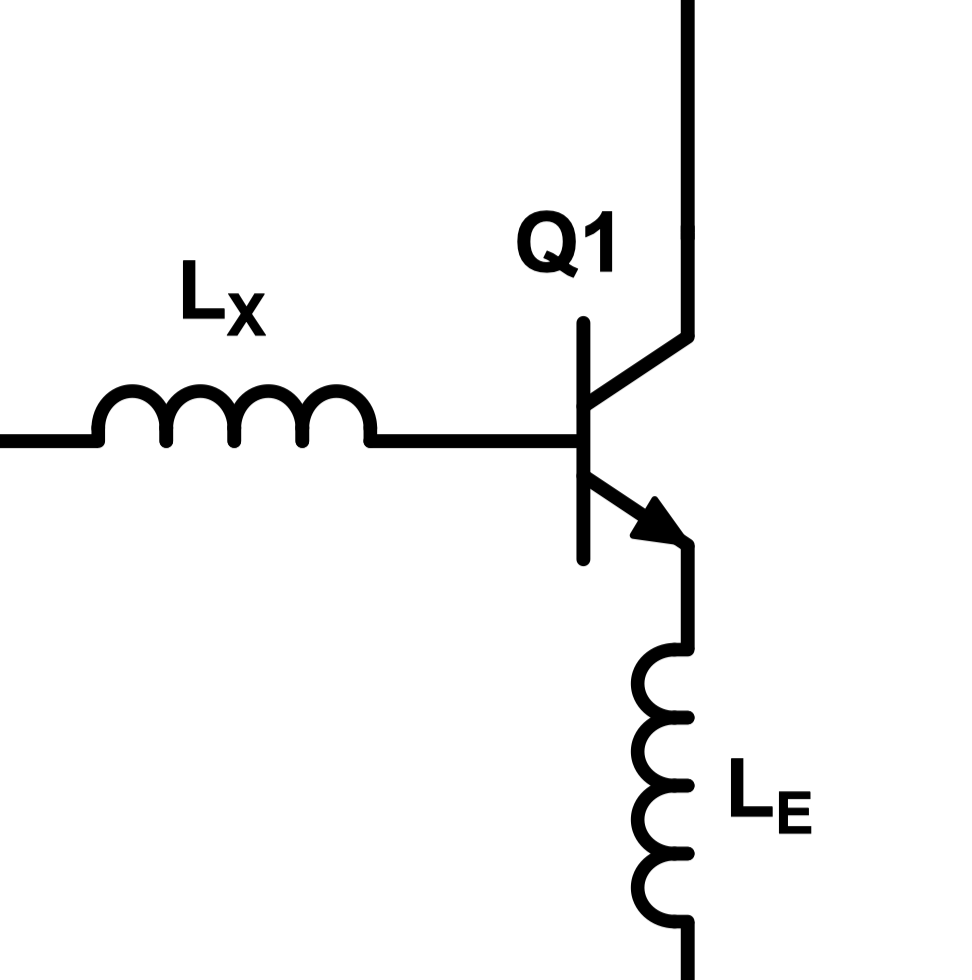
\includegraphics[scale=0.46]{fig/L_im.png}
\caption{}\label{fig:L_im}
\end{figure}


\[
L_E = \frac{R_s - r_{bb'}}{\omega_T} \simeq \frac{R_s}{\omega_T} 
\]

\[
L_B = \frac{1}{\omega_0^2 \cdot C_{\pi}} - L_E %= \frac{1}{\omega_0^2 \cdot \frac{g_m}{\omega_T}} = \frac{1}{\omega_0^2 \cdot \frac{I_C}{V_T \cdot \omega_T}}
\]
where 
\[
\omega_T = \frac{g_m}{C_{\pi}} \Rightarrow C_{\pi} = \frac{g_m}{\omega_T}
\]
and 
\[
g_m := \frac{\partial i_C}{\partial v_{be}} = \frac{I_C}{V_T }
\]


\end{document}